\documentclass[a4paper]{article}

%% Language and font encodings
\usepackage[english]{babel}
% \usepackage[utf8x]{inputenc}
\usepackage[T1]{fontenc}

%% Sets page size and margins
\usepackage[a4paper,top=3cm,bottom=2cm,left=3cm,right=3cm,marginparwidth=1.75cm]{geometry}

%% Useful packages
\usepackage{amsmath}
\usepackage{graphicx}
\usepackage[colorinlistoftodos]{todonotes}
\usepackage[colorlinks=true, allcolors=blue]{hyperref}

\usepackage{graphics}
\usepackage{epsfig} 
\usepackage{mathptmx} 
% \usepackage{times} 
\usepackage{amssymb}
\usepackage{array}
\usepackage{subcaption}

\title{\date{\vspace{-5ex}}
Homework 2 - Canny Edge Detection \\
}



\begin{document}
\maketitle
\thispagestyle{empty}
\pagestyle{empty}

\section{Canny Edge}

\textbf{1.1 Image Gradients} (2 points)\\
If a pixel located at $(x, y)$ has the horizontal derivative of $4$ ($I_x(x,\ y) = 4$) and the vertical derivative of $0$ ($I_y(x,\ y) = 0$), what is the gradient magnitude and orientation at $(x, y)$?\\
\vspace{10mm}

\noindent  \textbf{1.2 Edge Orientation} (2 points)\\
If there is an edge passes through the pixel $(x,y)$, then what's the edge orientation?\\
\vspace{10mm}

\noindent \textbf{1.3 Non-Maximum Suppression} (3 points)\\
% \subsection{Non-Maximum Suppression}
Given the gradient magnitudes and orientations, perform non-maximum suppression to compute the binary edge map. Write a ``+'' for pixels that remain in the edge map and leave blank cells for pixels that are suppressed.

\begin{figure}[!h]
	\begin{subfigure}{.5\textwidth}
	\centering
\begin{tabular}{|c|c|c|c|}
	\hline
	0 & 2 & 12 & 16   \\ \hline
	4 & 9 & 11 & 8   \\ \hline
	7 & 17 & 12 & 9   \\ \hline
	0 & 19 & 21 & 17   \\ \hline
\end{tabular}
\caption{Gradient magnitudes}
\end{subfigure}
	\begin{subfigure}{.5\textwidth}
	\centering
\begin{tabular}{|c|c|c|c|}
	\hline
	90^{\circ} & 45^{\circ} & 0^{\circ} & 45^{\circ}   \\ \hline
	45^{\circ} & 45^{\circ} & 45^{\circ} & 90^{\circ}   \\ \hline
	45^{\circ} & 0^{\circ} & 90^{\circ} & 45^{\circ}   \\ \hline
	90^{\circ} & 45^{\circ} & 90^{\circ} & 45^{\circ}   \\ \hline
\end{tabular}
	\caption{Gradient orientations in degrees}
\end{subfigure}

\end{figure}

\begin{figure}[!h]
	\centering
	
\begin{tikzpicture}
		\draw[step=1cm,gray,very thin] (-2,-2) grid (2,2);
	\end{tikzpicture}
	\caption{Binary edge map after non-maximum suppression}
\end{figure}


\newpage
\noindent \textbf{1.4 Hysteresis} (3 points).\\
Given the strong edge map (generated via the higher thresholding value), weak edge map (generated via the lower thresholding value), and gradient orientations, perform hysteresis and fill in the final edge map. Make note about X and Y.

\noindent\textbf{Note:} 1) the binary map is scanned in a row-major manner; 2) mark the edge point from the strong edge map with X and the other by Y.

\begin{figure}[!h]
	\begin{subfigure}{.5\textwidth}
	\centering
\begin{tabular}{|c|c|c|c|c|c|c|c|}
	\hline
0 & 0 & 0 & 0 & 0 & 0 & 0 & 0 \\ \hline
0 & 1 & 0 & 0 & 0 & 1 & 1 & 0 \\ \hline
0 & 1 & 0 & 0 & 0 & 1 & 0 & 0 \\ \hline
0 & 0 & 0 & 0 & 1 & 1 & 0 & 0 \\ \hline
0 & 0 & 0 & 0 & 0 & 0 & 0 & 0 \\ \hline
0 & 0 & 0 & 0 & 0 & 0 & 0 & 0 \\ \hline
0 & 0 & 0 & 0 & 0 & 0 & 0 & 0 \\ \hline
0 & 0 & 0 & 0 & 0 & 0 & 0 & 0 \\ \hline
\end{tabular}
\caption{Strong edge map}
\end{subfigure}
	\begin{subfigure}{.5\textwidth}
	\centering
\begin{tabular}{|c|c|c|c|c|c|c|c|}
	\hline
0 & 1 & 0 & 0 & 0 & 0 & 1 & 1 \\ \hline
0 & 1 & 0 & 0 & 0 & 1 & 1 & 0 \\ \hline
0 & 1 & 0 & 0 & 0 & 1 & 0 & 0 \\ \hline
0 & 1 & 0 & 0 & 1 & 1 & 0 & 0 \\ \hline
0 & 1 & 0 & 0 & 1 & 0 & 0 & 0 \\ \hline
0 & 0 & 1 & 0 & 0 & 0 & 0 & 0 \\ \hline
0 & 1 & 0 & 0 & 0 & 0 & 0 & 1 \\ \hline
0 & 1 & 0 & 0 & 0 & 0 & 1 & 1 \\ \hline
\end{tabular}
	\caption{Weak edge map}
\end{subfigure}

\begin{subfigure}{\textwidth}
	\centering
\begin{tabular}{|c|c|c|c|c|c|c|c|}
\hline
$0^{\circ}$ & $0^{\circ}$ & $0^{\circ}$ & $0^{\circ}$ & $45^{\circ}$ & $45^{\circ}$ & $45^{\circ}$ & $45^{\circ}$\\ \hline
$0^{\circ}$ & $0^{\circ}$ & $0^{\circ}$ & $0^{\circ}$ & $45^{\circ}$ & $45^{\circ}$ & $45^{\circ}$ & $45^{\circ}$\\ \hline
$0^{\circ}$ & $0^{\circ}$ & $0^{\circ}$ & $0^{\circ}$ & $45^{\circ}$ & $45^{\circ}$ & $45^{\circ}$ & $45^{\circ}$\\ \hline
$0^{\circ}$ & $0^{\circ}$ & $0^{\circ}$ & $0^{\circ}$ & $45^{\circ}$ & $45^{\circ}$ & $45^{\circ}$ & $45^{\circ}$\\ \hline
$0^{\circ}$ & $0^{\circ}$ & $0^{\circ}$ & $0^{\circ}$ & $45^{\circ}$ & $45^{\circ}$ & $45^{\circ}$ & $45^{\circ}$\\ \hline
$0^{\circ}$ & $0^{\circ}$ & $0^{\circ}$ & $0^{\circ}$ & $45^{\circ}$ & $45^{\circ}$ & $45^{\circ}$ & $45^{\circ}$\\ \hline
$0^{\circ}$ & $0^{\circ}$ & $0^{\circ}$ & $0^{\circ}$ & $45^{\circ}$ & $45^{\circ}$ & $45^{\circ}$ & $45^{\circ}$\\ \hline
$0^{\circ}$ & $0^{\circ}$ & $0^{\circ}$ & $0^{\circ}$ & $45^{\circ}$ & $45^{\circ}$ & $45^{\circ}$ & $45^{\circ}$\\ \hline

\end{tabular}
	\caption{Gradient orientation}
\end{subfigure}

\end{figure}

\begin{figure}[!h]
	\centering
	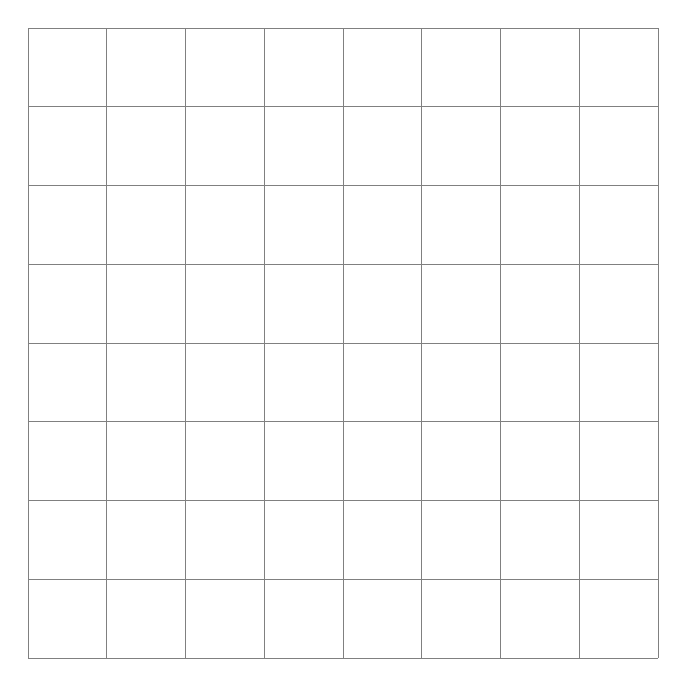
\begin{tikzpicture}
		\draw[step=1cm,gray,very thin] (-2,-2) grid (6,6);
	\end{tikzpicture}
	\caption{Final edge map}
\end{figure}



\end{document}